% Origen: sección "Apéndice" de Secciones/PI - Implementacion Multitrigger.md
% (Detalles de los submódulos, Mapa de memoria y Verificación).
\chapter{Detalles del multitrigger}
\label{C:ap-mt}

% Figuras de este apéndice + las compartidas.
\graphicspath{{figs/apendices/}{figs/comunes/}}

\section{Detalles de los submódulos}
\label{S:ap-mt-submodulos}

A continuación se presentan las decisiones de diseño de los submódulos con
lógica propia. Los puertos, registros y latencias de cada uno están en su hoja
de datos, en \ruta{prj/MCA/docs/datasheet} del repositorio, y el
\emph{ground truth} es el RTL, en \ruta{prj/MCA/modulos/mt}
\textbf{\textcolor{red}{(AGREGAR LINK)}}. En la Fig.~\ref{f:ap-mt-interfaz} se
presenta la interfaz del módulo completo.

\begin{figure}[H]
\centering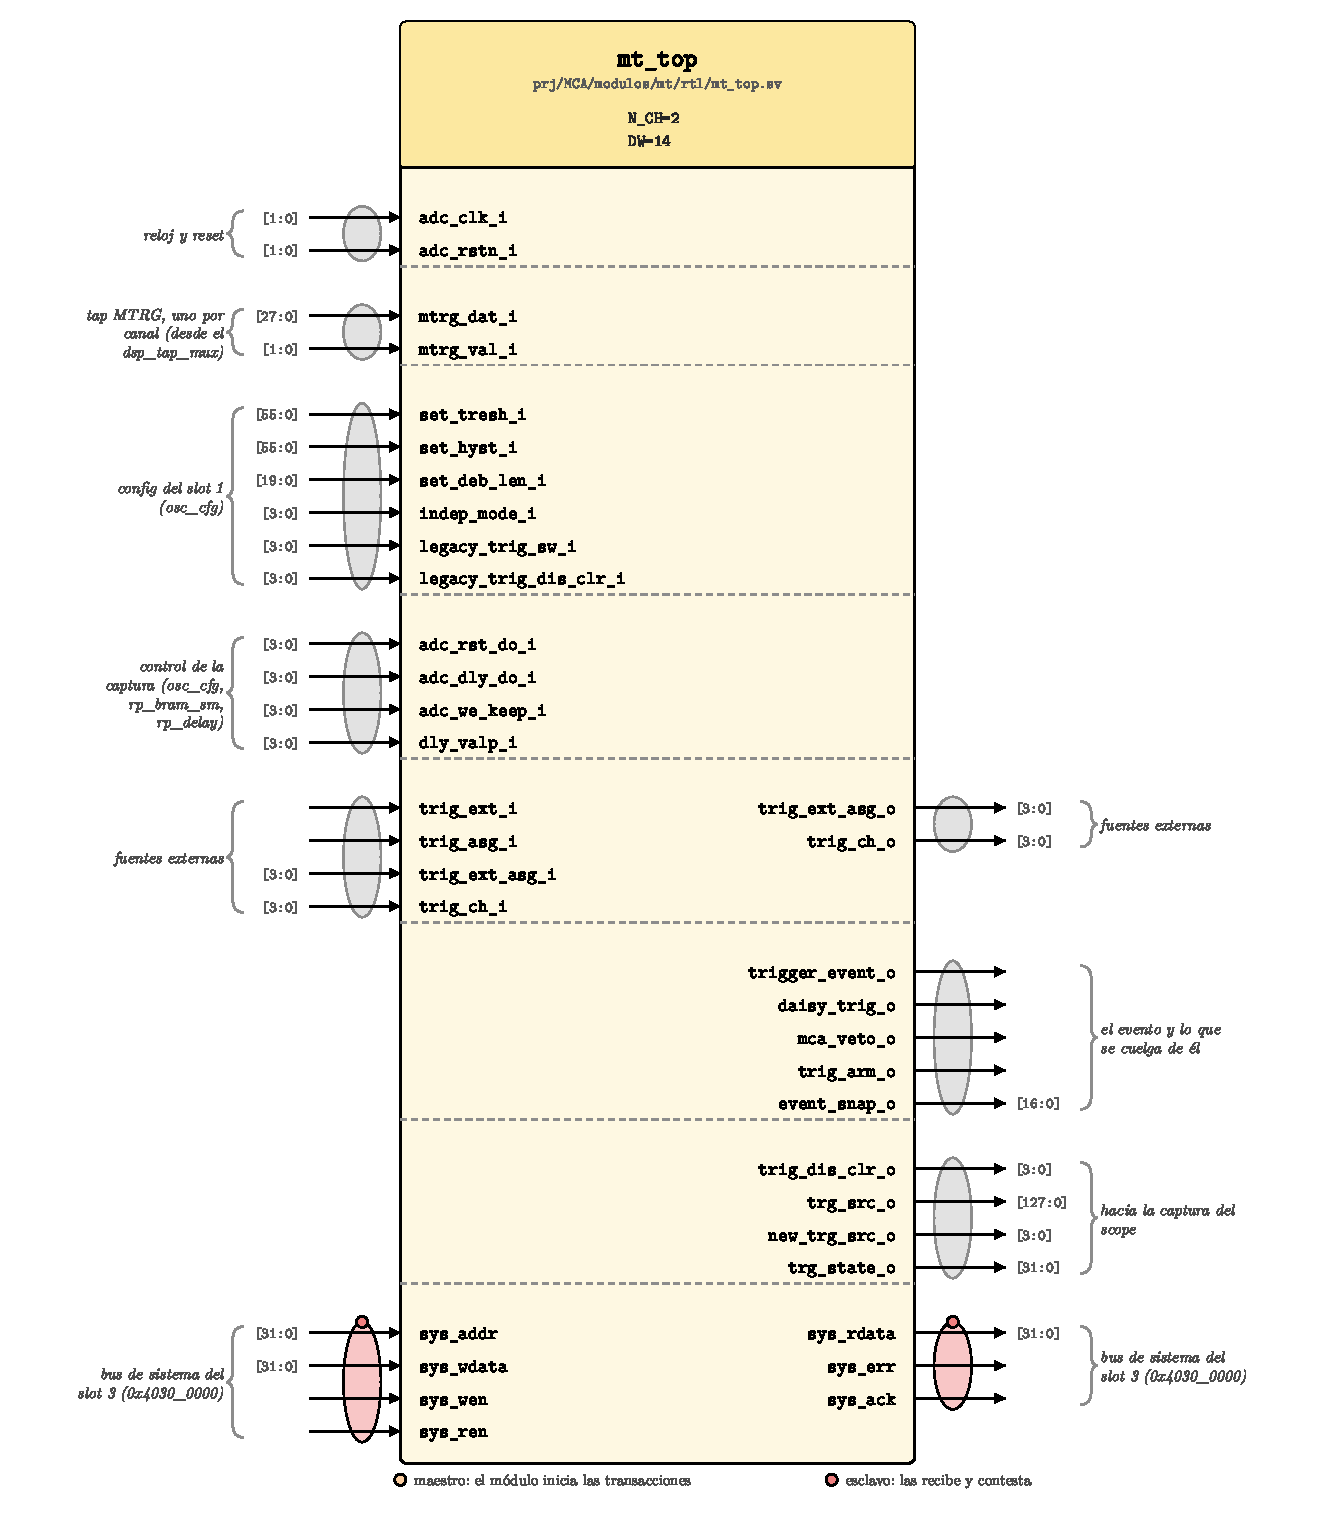
\includegraphics{apC_mt_top_interfaz}
\caption[Interfaz del multitrigger]{%
Interfaz del multitrigger, \codigo{mt\_top}.\label{f:ap-mt-interfaz}}
\end{figure}

\subsection{Disparo por pendiente \texorpdfstring{\texttt{mt\_slope\_trig}}{mt\_slope\_trig}}
\label{S:ap-mt-slope}

Compara el umbral contra una derivada suavizada de la
señal~\cite{Jordanov1994,CAENWP2081}, en lugar de la muestra:
\begin{equation}
  s[n] = \sum_{i=0}^{L-1} x[n-i] - \sum_{i=0}^{L-1} x[n-L-G-i]
  \label{e:ap-mt-slope}
\end{equation}
la suma de las últimas $L$ muestras menos la de $L$ muestras ubicadas $G$ más
atrás. La suma de sus coeficientes es cero, así que una continua da $s = 0$ y el
umbral efectivo no se mueve con la línea de base, como sí le pasa al disparo por
nivel. A la salida tiene un comparador con histéresis simétrico, que da un pulso
por pendiente positiva y otro por negativa.

Se calcula de forma recursiva~\cite{Jordanov1994b},
$s[n] = s[n-1] + (x[n] - x[n-L]) - (x[n-L-G] - x[n-2L-G])$, con tres líneas de
retardo en cascada ($L$, $G$ y $L$ muestras) de una sola toma cada una, que la
síntesis implementa como registros de desplazamiento~\cite{UG474}. Las líneas
avanzan sólo con la muestra válida (\codigo{adc\_dv\_i}), así que el filtro
funciona igual sobre la señal decimada que a 125~MS/s. No tienen \emph{reset}: un
contador \codigo{fill} cuenta las muestras que entraron desde el último
re-arranque, y una toma más vieja que eso lee 0. Así $s$ es exactamente el
filtro aplicado a una señal sin historia previa, y mientras la ventana de
$2L + G$ muestras no se llena no sale ningún pulso.

\begin{figure}[H]
\centering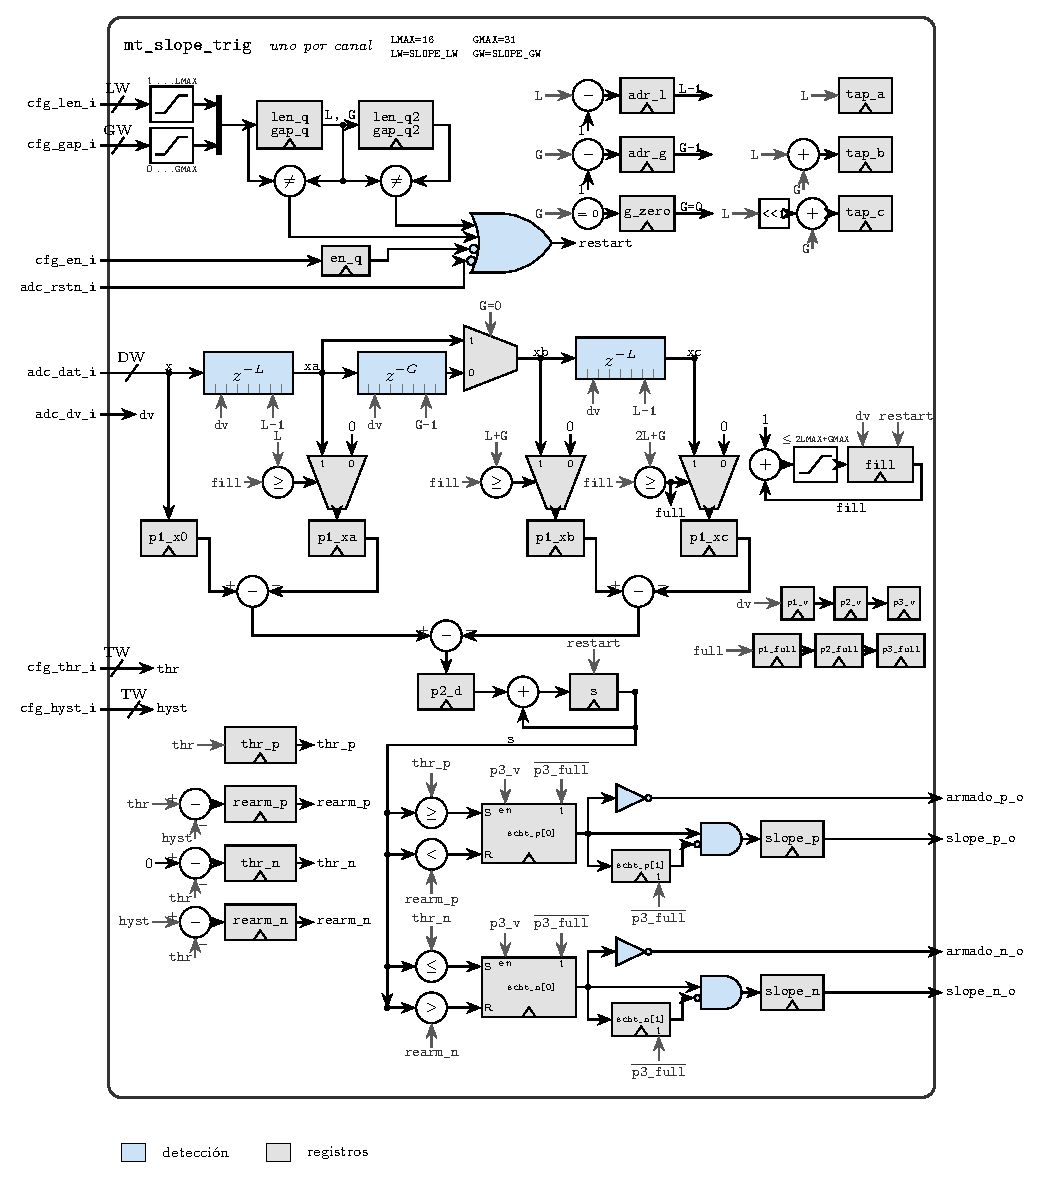
\includegraphics{apC_panorama_mt_slope_trig}
\caption[Implementación del disparo por pendiente]{%
Implementación de \codigo{mt\_slope\_trig}: las tres líneas de retardo, el
cálculo recursivo de $s$ y el comparador con histéresis.\label{f:ap-mt-slope}}
\end{figure}

\subsection{Disparo por polo-cero \texorpdfstring{\texttt{mt\_pz\_trig}}{mt\_pz\_trig}}
\label{S:ap-mt-pz}

Compara el umbral contra la salida de un trapecio corto con cancelación del
polo de la cola~\cite{Jordanov1994,Nakhostin2017}. Es el mismo
\codigo{mca\_trap} del MCA, con subida $k$ y meseta $m$ chicas y las líneas de
retardo en LUT, sin BRAM. Cada pulso sale como un trapecio que vuelve a cero a
las $2k + m$ muestras, apoyado en cero aunque haya una cola debajo. Por eso
separa pulsos cercanos y ve un pulso chico sobre la cola de uno grande, donde la
pendiente queda ciega porque no cancela el polo. El trapecio se presenta en la
Sec.~\refpend{S:implmca-trapezoidal}{Implementación del MCA: recuperación por
conformación trapezoidal}; a la salida tiene el mismo comparador con histéresis
que la pendiente, sólo para pulsos positivos.

\subsection{Escudo \texorpdfstring{\texttt{trigger\_shield}}{trigger\_shield}}
\label{S:ap-mt-shield}

Cuando dispara una fuente habilitada en \codigo{SHIELD\_SRC}, deja inhabilitados
a los destinos de \codigo{SHIELD\_DST} durante un \emph{holdoff} programable, y al
expirar los vuelve a armar. Usa un solo contador para todos los destinos, que se
recarga con cada disparo de una fuente. Fuentes y destinos son vectores
independientes: las fuentes son los disparos de los canales y la entrada
externa (flancos y nivel), y los destinos, los canales y el MCA. Con el mismo
contador resuelve dos cosas: que un canal no se re-dispare con su propio pulso
(Sec.~\ref{S:mt-vulnerabilidades}) y el veto al MCA. Con el nivel externo como
fuente, el veto dura lo que la línea más el \emph{holdoff}.

\begin{figure}[H]
\centering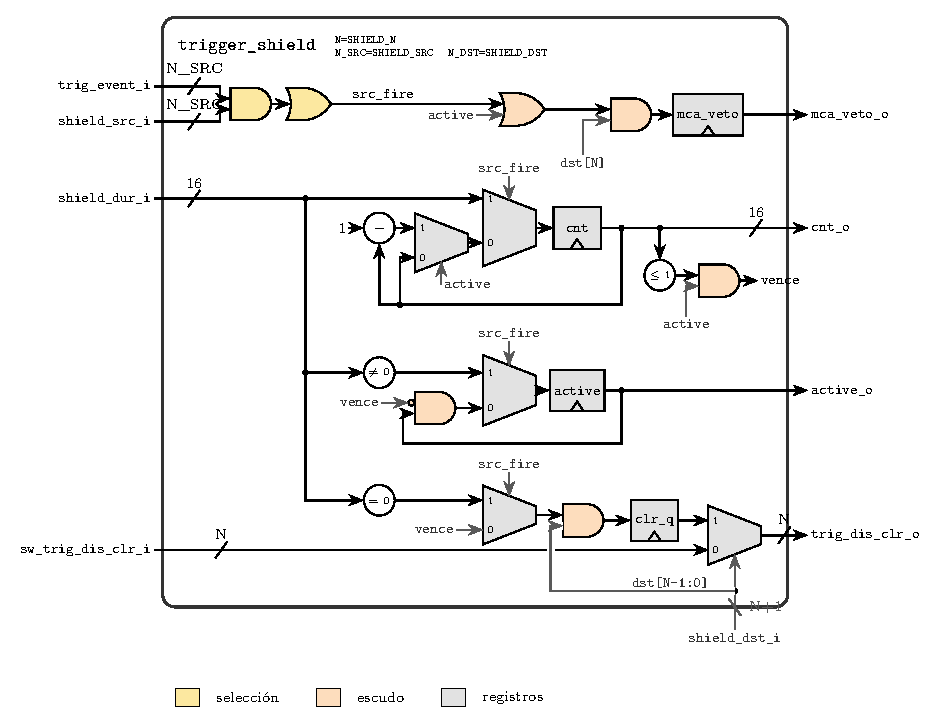
\includegraphics{apC_panorama_trigger_shield}
\caption[Implementación del escudo]{%
Implementación de \codigo{trigger\_shield}: el contador de \emph{holdoff}, el pulso de
re-armado hacia los canales y el veto al MCA.\label{f:ap-mt-shield}}
\end{figure}

\subsection[Selección de fuentes \texttt{mt\_trig\_src} y lógica de eventos \texttt{mt\_event\_logic}]{Selección de fuentes \texorpdfstring{\texttt{mt\_trig\_src}}{mt\_trig\_src}\texorpdfstring{\\}{} y lógica de eventos \texorpdfstring{\texttt{mt\_event\_logic}}{mt\_event\_logic}}
\label{S:ap-mt-src-logica}

\codigo{mt\_trig\_src} y \codigo{mt\_event\_logic} no tienen figura propia: su
estructura se ve en la Fig.~\ref{f:mt-panorama}.

\codigo{mt\_trig\_src} es el selector de un canal. Reemplaza al
\codigo{rp\_trig\_src} original~\cite{RedPitayaFPGA} con dos diferencias: la
máscara es una OR y no un selector de una sola fuente, y la salida va
registrada. Al disparar engancha \codigo{adc\_trg\_dis}, que impide que el
flanco siguiente vuelva a disparar hasta el \emph{clear}, que da el software o el
escudo al expirar su \emph{holdoff}. En \emph{single-shot} además limpia la máscara; en modo
continuo la máscara persiste y alcanza con el \emph{clear}.

\codigo{mt\_event\_logic} no tiene lógica de disparo propia. Instancia un
\codigo{mt\_trig\_src} por canal y el escudo, y saca el evento conjunto
(\codigo{trigger\_event}, la OR de los disparos de los canales),
\codigo{trig\_arm} y el \emph{snapshot} de las fuentes que dispararon el último evento.
El \emph{snapshot} toma las fuentes retrasadas un ciclo, para alinearlas con el
registro de \codigo{mt\_trig\_src}; sin ese retardo guardaría las del ciclo
equivocado.

\subsection{Configuración \texorpdfstring{\texttt{mt\_cfg}}{mt\_cfg}}
\label{S:ap-mt-cfg}

Sigue la estructura del módulo de configuración de la
Sec.~\ref{S:intro-hw-modulo-config}, y sus registros se presentan en la Tabla~\ref{t:ap-mt-mapa}.
Estos registros vivían en el bus del osciloscopio, mezclados con los suyos y
atados a su misma respuesta; pasarlos a un bus propio le da al multitrigger su
propio borde.

\section{Mapa de memoria}
\label{S:ap-mt-mapa}

En la Tabla~\ref{t:ap-mt-mapa} se presentan los registros del multitrigger con
su desplazamiento respecto de la base del módulo. Los registros por canal se repiten cada 4
bytes, de ch0 a ch3. Con todos los registros en su valor de \emph{reset} el módulo no
dispara: el disparo por software también pasa por la máscara (es el bit 0 de
\codigo{OR\_MASK}).

\begin{table}[H]
\centering
\caption[Mapa de registros del multitrigger]{%
Mapa de registros del multitrigger.\label{t:ap-mt-mapa}}
\footnotesize
\setlength{\tabcolsep}{3pt}
\begin{tabularx}{\textwidth}{|>{\raggedright\arraybackslash}p{0.13\textwidth}|c|l|>{\raggedright\arraybackslash}X|>{\raggedright\arraybackslash}p{0.15\textwidth}|}
\hline
\encabezado \textbf{\emph{Offset}} & \textbf{Acceso} & \textbf{Registro}
  & \textbf{Contenido} & \textbf{\emph{Reset}} \\ \hline
\codigo{0x000} & R & \codigo{MAGIC}
  & \codigo{0x4D545247} (\codigo{\textquotedbl MTRG\textquotedbl}) & constante \\ \hline
\codigo{0x004} & R & \codigo{CAPS}
  & \codigo{\{HAS\_PZ[17], HAS\_SLOPE[16], SHIELD\_N[15:12], SRC\_W[11:4],
    N\_CH[3:0]\}} & constante \\ \hline
\codigo{0x010} & RW & \codigo{SHIELD\_CFG}
  & \codigo{\{dur[31:16], dst[12:8], src[6:0]\}} & \codigo{0}, escudo apagado
  \\ \hline
\codigo{0x014} & R & \codigo{SHIELD\_STAT}
  & \codigo{\{trig\_arm[18], mca\_veto[17], active[16], cnt[15:0]\}}
  & \codigo{0} \\ \hline
\codigo{0x018} & R & \codigo{SNAPSHOT}
  & fuentes que dispararon el último evento (29~b) & \codigo{0} \\ \hline
\codigo{0x01C} & R & \codigo{DIS\_FLAGS}
  & \codigo{\{we\_keep[7:4], dis\_act[3:0]\}} & \codigo{0} \\ \hline
\codigo{0x020} & W & \codigo{TRIG\_SW}
  & disparo por software, un bit por canal & lee \codigo{0} \\ \hline
\codigo{0x024} & W & \codigo{TRIG\_DIS\_CLR}
  & \emph{clear} del enganche, un bit por canal & lee \codigo{0} \\ \hline
\codigo{0x028} & R & \codigo{TRG\_STATE}
  & máscara activa, 8~b por canal & \codigo{0} \\ \hline
\codigo{0x040}~+~4$\cdot$ch & RW & \codigo{OR\_MASK}
  & máscara OR del canal, un bit por fuente & \codigo{0}, no dispara nada \\ \hline
\codigo{0x060}~+~4$\cdot$ch & RW & \codigo{SLOPE\_CFG}
  & \codigo{\{en[31], G[12:8], L[4:0]\}} & \codigo{0}, apagado \\ \hline
\codigo{0x070}~+~4$\cdot$ch & RW & \codigo{SLOPE\_THR}
  & umbral de la pendiente \codigo{[17:0]} & \codigo{0} \\ \hline
\codigo{0x080}~+~4$\cdot$ch & RW & \codigo{SLOPE\_HYST}
  & histéresis de la pendiente \codigo{[17:0]} & \codigo{0} \\ \hline
\codigo{0x090}~+~4$\cdot$ch & RW & \codigo{PZ\_CFG}
  & \codigo{\{en[31], sh[29:24], m[12:8], k[4:0]\}} & \codigo{0}, apagado \\ \hline
\codigo{0x0A0}~+~4$\cdot$ch & RW & \codigo{PZ\_MQ}
  & constante del polo-cero, $16 M$ \codigo{[19:0]} & \codigo{0} \\ \hline
\codigo{0x0B0}~+~4$\cdot$ch & RW & \codigo{PZ\_THR}
  & umbral del polo-cero \codigo{[17:0]} & \codigo{0} \\ \hline
\codigo{0x0C0}~+~4$\cdot$ch & RW & \codigo{PZ\_HYST}
  & histéresis del polo-cero \codigo{[17:0]} & \codigo{0} \\ \hline
\end{tabularx}
\end{table}

\section{Verificación}
\label{S:ap-mt-verificacion}

En la Tabla~\ref{t:ap-mt-tests} se presentan los \emph{testbenches} del módulo. Los dos
disparos con filtro se comparan contra un modelo de referencia (\emph{golden
model})~\cite{Bergeron2003} en cada ciclo; el resto se verifica con casos
dirigidos, cada uno con su valor esperado. \codigo{tb\_mt\_top} prueba el módulo
entero a través de su borde, es decir, el cableado entre los submódulos.

\begin{table}[H]
\centering
\caption[\emph{Testbenches} del multitrigger]{%
\emph{Testbenches} del multitrigger.\label{t:ap-mt-tests}}
\footnotesize
\setlength{\tabcolsep}{3pt}
\begin{tabularx}{\textwidth}{|>{\raggedright\arraybackslash}p{0.2\textwidth}|>{\raggedright\arraybackslash}X|>{\raggedright\arraybackslash}p{0.2\textwidth}|}
\hline
\encabezado \textbf{\emph{Testbench}} & \textbf{Qué verifica} & \textbf{Referencia} \\ \hline
\codigo{tb\_mt\_slope\_trig} & el filtro y los pulsos por escalón; que ni la
  continua ni una rampa lenta disparen; el re-arranque al cambiar $L$ o $G$; la
  señal de re-armado & modelo de suma directa \\ \hline
\codigo{tb\_mt\_pz\_trig} & el trapecio y el comparador; el arranque con
  continua; el re-arranque; pares de pulsos; la señal decimada; la señal de
  re-armado & modelo del trapecio y del comparador, bit a bit \\ \hline
\codigo{tb\_mt\_trig\_src} & la máscara OR; el enganche \codigo{adc\_trg\_dis}
  y su \emph{clear}; el disparo por software sujeto a \codigo{dly\_valp}; las fuentes
  de pendiente y polo-cero & casos dirigidos \\ \hline
\codigo{tb\_trigger\_shield} & el \emph{holdoff} de fuentes a destinos, con
  \codigo{dur = 0} y con \codigo{dur} $>$ 0 & casos dirigidos \\ \hline
\codigo{tb\_mt\_event\_logic} & \codigo{trigger\_event} como OR de los canales;
  el \emph{snapshot} (enganche, borrado, alineación con el evento); que un
  \codigo{TRIG\_SW} dé un solo evento; \codigo{trig\_arm} con la máscara vacía,
  fuentes fuera de la máscara, el re-armado y el enganche del escudo
  & casos dirigidos \\ \hline
\codigo{tb\_mt\_cfg} & cada registro contra el mapa anterior; los accesos
  heredados del bus del osciloscopio; el \emph{fan-out} entre canales; el contrato del
  bus en todo su espacio de direcciones & mapa de registros anterior \\ \hline
\codigo{tb\_mt\_top} & cada tipo de disparo configurado por registros hasta
  \codigo{trigger\_event} (nivel, pendiente, polo-cero, externo, software,
  cadena); el veto por nivel externo; el modo continuo; el lazo con la captura;
  \codigo{trig\_arm} & casos dirigidos \\ \hline
\end{tabularx}
\end{table}

% Las figuras y tablas son más largas que el texto: sin el \clearpage flotan
% detrás de las referencias.
\clearpage
\bibliografiacapitulo

%%% Local Variables:
%%% mode: latex
%%% TeX-master: "template"
%%% End:
